\section[Nó Cliente]{Nó Cliente: Pipeline de Processamento de Imagens e Extração de Características}

Nesta seção, é detalhado o pipeline de processamento de imagens implementado na camada de borda do sistema. Essa etapa é responsável pela captura contínua dos frames, detecção da face, extração da região de interesse (ROI), verificação da qualidade da amostra facial e geração do vetor de características por meio do modelo ArcFace.
\subsection{Pipeline de Visão Computacional}

O fluxo de processamento de dados biométricos foi estruturado para assegurar eficiência, qualidade da amostra e confiabilidade na comunicação com os serviços remotos. O processo é composto por cinco etapas principais, representadas na Figura~\ref{fig:fluxograma_PDI}:
\begin{figure}[htbp]
    \centering
    \caption{Funcionamento da pipeline de processamento de imagens e extração de características faciais.}
    \vspace{-10pt}
    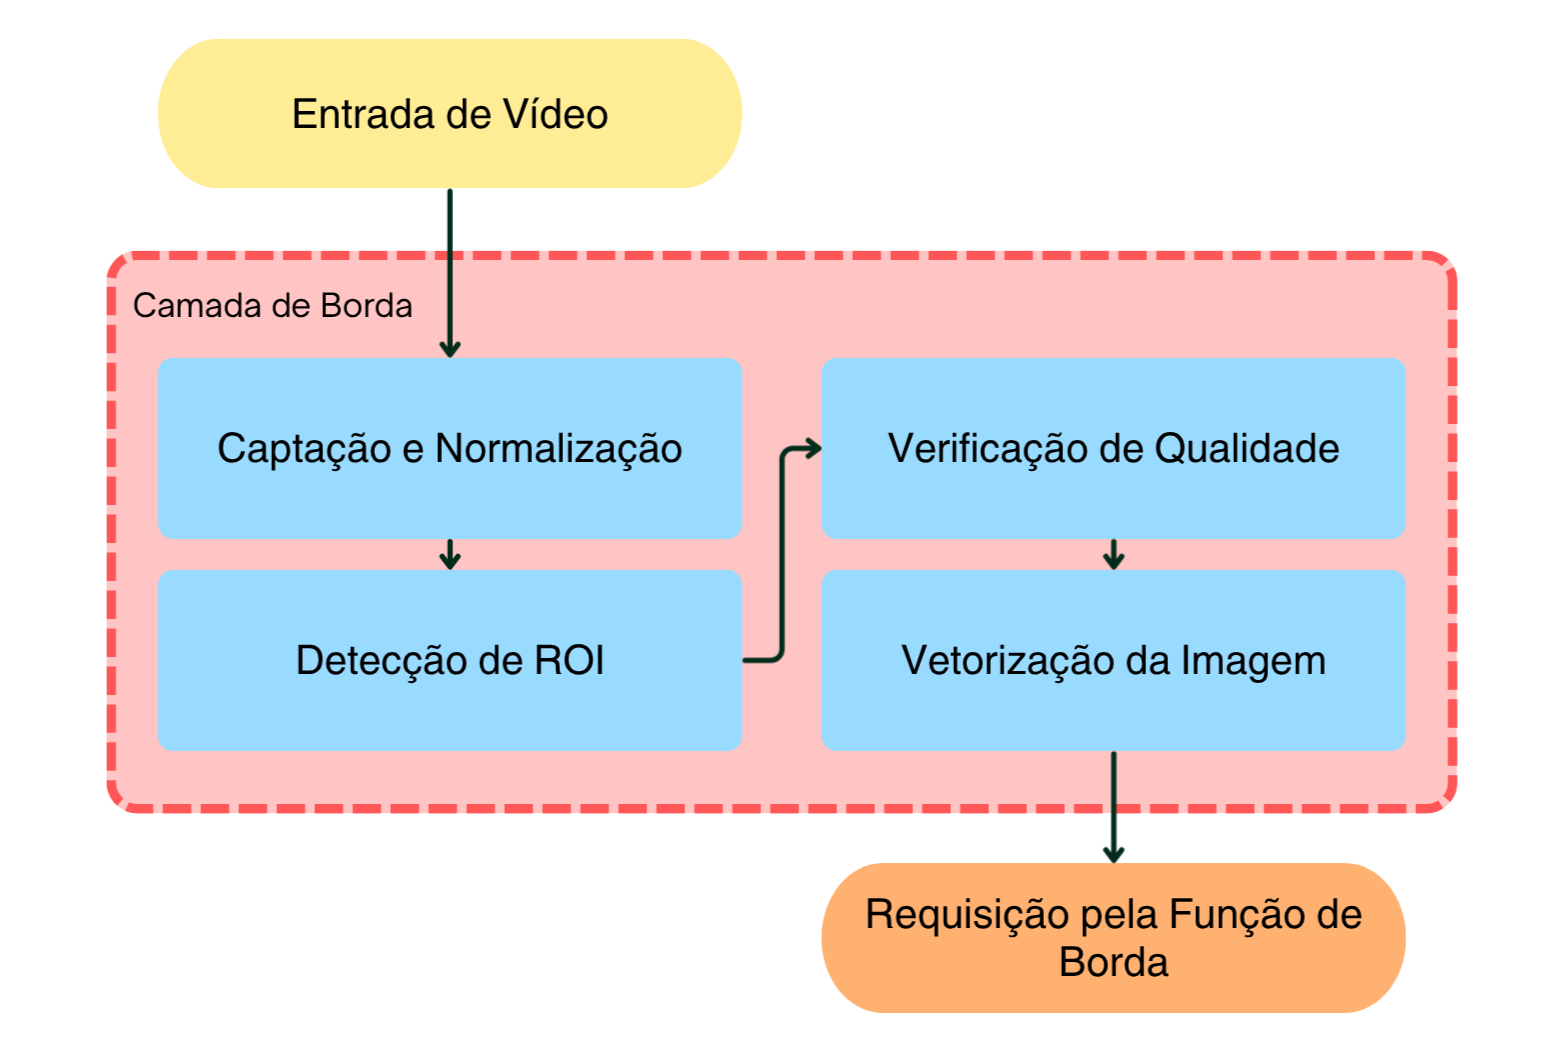
\includegraphics[width=0.8\textwidth ,  keepaspectratio]{images/flowchartPDI.png}
    \par\vspace{6pt} % Pequeno espaçamento opcional entre a imagem e a legenda
    \label{fig:fluxograma_PDI}
    \footnotesize Fonte: Elaborada pelo autor.
\end{figure}




\subsubsection{Descrição das Etapas}

\begin{enumerate}
    \item \textbf{Captação e Normalização:} O sistema inicia com a captura do fluxo de vídeo por meio da interface \texttt{cv2.VideoCapture}. Os frames capturados são utilizados como entrada para o modelo de detecção facial, permitindo a análise contínua da cena em tempo real. Essa etapa padroniza o fluxo de entrada do sistema e estabelece a base para as etapas seguintes de detecção, recorte e validação da face.

    \item \textbf{Detecção e Extração de ROI:} O modelo YOLO atua como detector primário, localizando a face no frame e retornando as coordenadas da caixa delimitadora. A partir dessas coordenadas, o sistema recorta a Região de Interesse (ROI), mantendo apenas a área facial para as etapas seguintes.

    \item \textbf{Auditoria de Qualidade:} Antes da vetorização, o recorte facial passa por uma verificação de qualidade. São avaliados critérios como área mínima da face, nível médio de brilho, confiança da detecção e nitidez estimada pelo operador Laplaciano. Apenas amostras que atendem aos limiares definidos no sistema prosseguem no \textit{pipeline}, evitando o envio de imagens muito pequenas, escuras, superexpostas ou borradas.
    
    \item \textbf{Vetorização (Embedding):} A face validada é convertida pelo modelo \textit{ArcFace} em um vetor numérico de alta dimensionalidade (\textit{embedding}), que sintetiza as características geométricas únicas do indivíduo para posterior comparação matemática.

    \item \textbf{Comunicação e Validação Remota:} O \textit{embedding}, a identificação da porta e o recorte facial codificado em Base64 são enviados para a infraestrutura em nuvem. Na etapa remota, o vetor é consultado no banco vetorial, a similaridade é avaliada e o sistema retorna ao ponto de origem o status da tentativa de acesso.
\end{enumerate}

\subsection{Isolamento da Região de Interesse (ROI):}

\subsubsection{Detecção de Faces com YOLOv8}
A detecção de rostos foi realizada utilizando a arquitetura YOLO (You Only Look Once), uma rede neural convolucional de estágio único que processa a imagem em uma única passagem direta \cite{redmon2016you}. A implementação baseou-se no framework Ultralytics YOLOv8 \cite{yolov8_ultralytics}, utilizado para localizar a face nos frames capturados e retornar as coordenadas da caixa delimitadora. Essa escolha é adequada para aplicações em tempo real, pois permite detectar a região facial com baixa latência antes da etapa de extração de características.

O conjunto de dados, composto pelas 2.800 imagens do \textit{FEI face database}, passou por um processo de normalização e anotação automatizada. O processo utilizou um modelo pré-treinado de detecção facial baseado em Caffe, pré-treinado com arquitetura ResNet-10 SSD, para delimitar as áreas de interesse em cada imagem, garantindo que apenas exemplos com detecções positivas compusessem a base final. O dataset foi, por fim, particionado para o treinamento e a validação da rede, seguindo a divisão de 80\% e 20\%, respectivamente.


\subsubsection{Resultados do Treinamento e Validação}
O modelo YOLOv8n foi treinado com \textit{batch size} 4, resolução de 416 pixels e ausência de \textit{data augmentation}. O processo estendeu-se por 87 épocas, com duração total de 4,6 horas e monitoramento contínuo das funções de perda (\textit{box loss}, \textit{cls loss} e \textit{dfl loss}) para garantir a convergência e evitar \textit{overfitting}.

Os resultados confirmaram a eficácia do modelo \textit{best.pt}, que atingiu \textit{mAP@50} de 0,995 e \textit{mAP@50-95} de 0,966, com latência de inferência de 19,5 ms por imagem, confirmando a robustez do sistema para aplicações de reconhecimento facial.


\subsection{Extração e Vetorização de Características Faciais}

Com a face detectada, recortada e validada, o sistema procede para a extração de características, convertendo a imagem em um vetor numérico de alta dimensionalidade, denominado \textit{embedding facial}. Esse processo é executado localmente por meio da biblioteca DeepFace utilizando o modelo \textit{ArcFace}. A vantagem dessa abordagem é substituir a comparação direta de pixels por uma comparação matemática entre vetores, tornando o processo de reconhecimento mais adequado a variações de iluminação, expressão facial e enquadramento \cite{deepfacegithub}.

A eficácia do \textit{ArcFace} reside na função de perda \textit{Additive Angular Margin Loss}, que otimiza a separação angular entre identidades diferentes. Enquanto modelos tradicionais baseados em \textit{softmax} limitam-se à classificação, o \textit{ArcFace} maximiza a distância entre classes distintas e minimiza a variação intra-classe no espaço angular, conforme definido pela Equação \ref{eq:FuncaoPerda}:

\begin{equation}
\label{eq:FuncaoPerda}
L = -\frac{1}{N}\sum_{i=1}^{N} \log \frac{e^{s\cos(\theta_{y_i}+m)}}{e^{s\cos(\theta_{y_i}+m)} + \sum_{j=1, j \neq y_i}^{n} e^{s\cos(\theta_j)}}
\end{equation}

Nesta expressão, \(N\) representa o número de amostras, \(y_i\) a classe correta, \(\theta_{y_i}\) o ângulo entre o vetor de características e o peso da classe, enquanto \(m\) e \(s\) representam a margem angular e o fator de escala, respectivamente \cite{deng2019arcface}. 

O resultado desse processo é um vetor de \textit{embedding facial} de 512 dimensões, conforme ilustrado na Tabela~\ref{tab:exemplo_embedding}, que encapsula as características faciais de forma compacta e discriminativa, permitindo a comparação eficiente com os vetores previamente cadastrados no banco de dados vetorial.


\begin{table}[htbp]
    \centering
    \caption{Exemplo da estrutura e valores do vetor de embedding gerado pelo modelo ArcFace.}
    \label{tab:exemplo_embedding}
    \vspace{6pt}
    \begin{tabular}{cc}
        \hline
        \textbf{Índice} & \textbf{Valor do Embedding} \\ \hline
        0  & -0.226871639 \\
        1  &  0.036645882 \\
        2  &  0.053239971 \\
        3  & -0.223227322 \\
        \vdots & \vdots \\
        510 &  0.07878179 \\
        511 & 0.078781798 \\ \hline

    \end{tabular}
\end{table}
